\section{Hyperparameter tuning}
\label{sec:tuning}

\paragraph{Protocol.} We tuned each model with Optuna and its TPE sampler
(seed 42, so a re-run proposes the same trials). One trial is one
configuration and one cross-validated score:
\begin{enumerate}
  \item Optuna proposes a set of hyperparameters;
  \item we build the complete Pipeline with them (features, preprocessing,
  model);
  \item we score it with the same 5-fold stratified cross-validation on the
  development set;
  \item Optuna receives the mean AP over the 5 folds, and uses all the past
  trials to choose the next configuration.
\end{enumerate}
The budget is 25 trials for the logistic regression, 20 for the random forest
(the slowest to fit) and 50 for LightGBM, which has the largest search space.
A grid search would not fit this budget: with only three values for each of
LightGBM's eight hyperparameters, it would need $3^8 = 6{,}561$
configurations, i.e.\ about 33{,}000 fits with 5-fold CV. A random search would
fit the budget, but it ignores the scores of past trials, whereas Optuna's TPE
sampler uses them to spend more trials in the promising regions of the space.
The search spaces are given in Table~\ref{tab:search-spaces} (appendix). They
include the class weighting (Section~\ref{sec:imbalance}), from no weight at
all up to the class ratio. We optimize AP because it judges the ranking of the
minority class without depending on a threshold, which is chosen afterwards.

\paragraph{Why the best CV score is optimistic.} The best of 20 to 50 trials is
selected on the same folds that score it, so part of its advantage is luck on
these particular folds. The best mean CV AP is therefore an optimistic estimate
of performance, and we do not report it as our final result: the honest
estimate comes from the test set, which played no role in tuning
(Section~\ref{sec:test}). Nested cross-validation would remove this bias
without a test set, but it would multiply the cost of tuning by five; with
48{,}790 rows, a held-out test set was the cheaper way to get an unbiased
estimate.

\paragraph{Final training.} For each model, \code{train.py} then
(1) computes the out-of-fold probabilities of the tuned Pipeline on the same 5
folds, (2) chooses the threshold that maximizes F1 on them and freezes it,
(3) refits the Pipeline on the whole development set, and (4) saves the fitted
Pipeline with its threshold. The final model is the one with the best
out-of-fold AP.

\paragraph{Results.} Table~\ref{tab:best-params} gives the best configuration
of each model and its mean CV AP.

\begin{table}[H]
\centering
\caption{Best hyperparameters found by Optuna and best mean CV AP.}
\label{tab:best-params}
\small
\begin{tabular}{lp{8.5cm}r}
\toprule
Model & Best hyperparameters & CV AP \\
\midrule
Logistic regression & $C = 1.89$, \code{l1\_ratio} $= 0.77$ (Elastic Net, mostly
Lasso), no class weight & 0.784 \\
Random forest & 200 trees, \code{max\_depth} $= 14$, \code{min\_samples\_leaf}
$= 3$, \code{max\_features} $= 0.60$, \code{class\_weight="balanced"} & 0.815 \\
LightGBM & 350 trees, learning rate $0.048$, 26 leaves,
\code{min\_child\_samples} $= 11$, \code{subsample} $= 0.81$,
\code{colsample\_bytree} $= 0.57$, $\lambda = 0.015$,
\code{scale\_pos\_weight} $= 1.80$ & 0.833 \\
\bottomrule
\end{tabular}
\end{table}

Three observations:
\begin{itemize}
  \item \textbf{Edges of the ranges.} Only one value landed at the edge of its
  range: \code{max\_features} $= 0.60$ for the random forest, the upper bound.
  Letting each split see more features might still help the forest a little;
  we did not extend the range because the forest stays well behind LightGBM.
  All the other values are inside their ranges.
  \item \textbf{Class weighting.} Optuna made three different choices: no
  weight for the logistic regression, \code{"balanced"} for the random forest,
  and a moderate weight of 1.80 for LightGBM, about half of the class ratio
  (3.2). Since the threshold is tuned afterwards in every case, the weight is
  just one more hyperparameter, kept only when it improves AP.
  \item \textbf{A flat optimum for LightGBM.} Its best trial is trial 2: the 47
  following trials did not beat it (Figure~\ref{fig:lgbm-history}). Many
  configurations reach about the same AP, so more trials would not change the
  model much.
  \item \textbf{The learning rate.} Its range, 0.01 to 0.2 on a log scale,
  covers the usual values, and the trials show why the optimum is flat. Below
  0.02, even 1{,}000 trees are not enough to finish learning (mean AP 0.811
  over 2 trials). Above 0.1, each tree corrects too much at once (mean AP
  0.826 over 21 trials). Between 0.02 and 0.1, the 27 trials average 0.829
  and the ten best all lie within 0.002 AP, about the variation across folds.
  The selected $\eta = 0.048$ with 350 trees is therefore one good point of a
  plateau rather than a sharp optimum; the number of trees was chosen by
  cross-validation together with $\eta$, not by early stopping.
\end{itemize}

\begin{figure}[H]
\centering
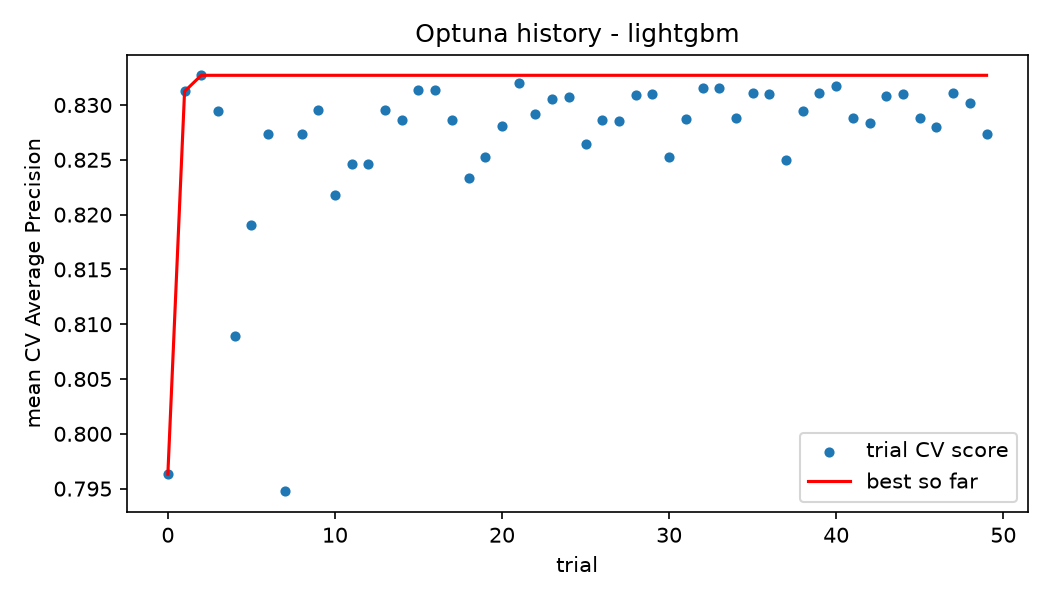
\includegraphics[width=0.65\textwidth]{lightgbm_history.png}
\caption{Mean CV AP of each Optuna trial for LightGBM.}
\label{fig:lgbm-history}
\end{figure}

\subsection{What the penalty does to the logistic regression}
\label{sec:regularization}

To see what the tuned penalty does, we look at the coefficients of the
final logistic regression and at the regularization path: train and validation
AP (5-fold CV, development set) for $C$ from $10^{-4}$ to $100$, with
\code{l1\_ratio} kept at its tuned value of 0.77
(Figure~\ref{fig:regularization-path}, script \code{src/regularization.py}).

\begin{itemize}
  \item \textbf{Sparsity.} The L1 part of the penalty sets 9 of the 91
  coefficients exactly to zero: seven \code{native-country} categories, mostly
  rare ones (Ecuador, Honduras, Holand-Netherlands, \dots), \code{workclass} =
  Never-worked, and \code{relationship} = Not-in-family, which carries
  little extra information once marital status and the other relationship
  categories are known. A Ridge penalty would only have shrunk them.
  \item \textbf{Strong penalty = underfitting.} At $C = 10^{-4}$ every
  coefficient is zero and the model predicts the base rate for everyone (AP
  0.24, the share of >50K). As $C$ grows, the model keeps more coefficients
  (7 at $C = 10^{-3}$, 39 at $C = 0.1$) and AP rises quickly.
  \item \textbf{Weak penalty does not overfit here.} Above $C \approx 0.1$
  the validation AP is flat (0.782 to 0.784), and the gap between train and
  validation AP stays below 0.004 even at $C = 100$. With about 39{,}000 rows
  for 91 coefficients, the model has too few parameters to memorize the
  training folds. This explains why tuning did not improve the logistic
  regression (Section~\ref{sec:models}): the tuned $C = 1.89$ lies in a
  flat region where the strength of the penalty barely matters.
  \item \textbf{A simpler model at almost no cost.} With $C = 0.1$, 39
  coefficients reach AP 0.782 against 0.784 with all 91. If a short, readable
  model mattered more than the last 0.002 AP, this stronger penalty would be
  the better choice.
\end{itemize}

\begin{figure}[H]
\centering
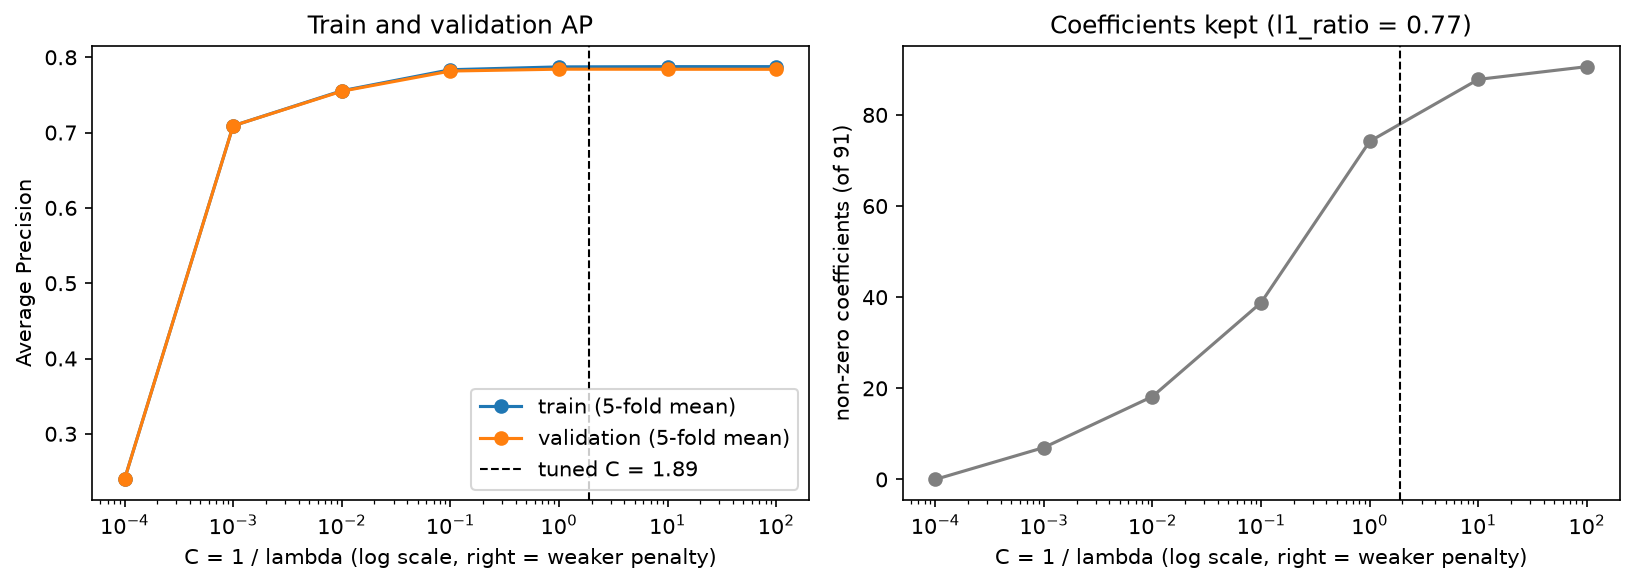
\includegraphics[width=\textwidth]{regularization_path.png}
\caption{Regularization path of the logistic regression (\code{l1\_ratio} =
0.77). Left: mean train and validation AP over the 5 folds. Right: mean number
of non-zero coefficients. Dashed line: the tuned $C$.}
\label{fig:regularization-path}
\end{figure}
